\documentclass[10pt,a4paper]{article}
\usepackage[utf8]{inputenc}
\usepackage[french]{babel}
\usepackage[T1]{fontenc}
\usepackage{amsmath}
\usepackage{amsfonts}
\usepackage{amssymb}
\usepackage{graphicx}
\usepackage[lofdepth,lotdepth]{subfig}
\usepackage[left=2cm,right=2cm,top=2cm,bottom=2cm]{geometry}
\usepackage{physics} %Physics.sty
\author{Loann Brahimi}
\title{Détermination du taux de turbulence des ondes de Alfvén par équilibre du taux de croissance et d'amortissement des ondes de Alfvén dans les milieux faiblement ionisés}
\begin{document}
\maketitle 

\section*{Coefficients d'amortissement par collisions ions-neutres}

Dans ce document nous allons calculer le coefficient d'amortissement des ondes de Alfvén par collisions des ions avec les neutres dans le cadre d'un milieu faiblement ionisé. On écrit dans un premier temps la relation de dispersion des ondes de Alfvén incluant un amortissement suivant les collisions neutre-ion et la viscosité des neutres. On a (Xu 2015) :

\begin{equation}
	\omega^3 + i\left({\tau_v}^{-1} + (1+\chi)\nu_{ni}\right)\omega^2 - \left(k^2\cos^2{\theta} {V_{Ai}}^2 + 
	\chi{\tau_v}^{-1}\nu_{ni}\right)\omega - i\left({\tau_v}^{-1} + \nu_{ni}\right)k^2\cos^2{\theta} {V_{Ai}}^2 = 0
	\label{1}
\end{equation}

où $\chi = \rho_n / \rho_i$ et ${\tau_v}^{-1} = k^2 \nu^n$. Dans un premier temps, on néglige la viscosité cinématique des neutres $\nu_n \approx 0$, l'équation \ref{1} devient : 

\begin{equation}
	\omega^3 + i(1+\chi)\nu_{ni}\omega^2 - k^2\cos^2{\theta} {V_{Ai}}^2\omega - i\nu_{ni}k^2\cos^2{\theta} {V_{Ai}}^2 = 0
	\label{2}
\end{equation}

Xu+2015 propose des solutions analytiques dans le cas d'un amortissement faible c'est à dire $\abs{\Gamma_{in}} \ll \abs{\omega_R}$. 

\begin{eqnarray}
	{\omega_R}^2 & = & \frac{k^2\cos^2{\theta}{V_{Ai}}^2 \left[(1+\chi){\nu_{ni}}^2 + k^2 \cos^2{\theta} {V_{Ai}}^2\right]}{(1+\chi)^2{\nu_{ni}}^2 + k^2 \cos^2{\theta} {V_{Ai}}^2} \\
	\Gamma_{in}  & = & - \frac{\nu_{ni}\chi  k^2 \cos^2{\theta} {V_{Ai}}^2}{2\left[ (1+\chi)^2{\nu_{ni}}^2 + k^2 \cos^2{\theta} {V_{Ai}}^2 \right]}
\end{eqnarray}

Dans le cas d'un couplage fort ($\omega \ll \nu_{in}$) on a : 

\begin{eqnarray}
	{\omega_{R,s}}^2 & = & {V_{A}}^2 k^2 \cos^2{\theta} \\ 
	\Gamma_{in,s}  & = & - \frac{\xi_n  {V_{A}}^2 k^2 \cos^2{\theta}}{2 \nu_{ni}}
\end{eqnarray}


Dans le cas d'un couplage faible ($\omega \gg \nu_{in}$) on a : 

\begin{eqnarray}
	{\omega_{R,w}}^2 & = & {V_{Ai}}^2 k^2 \cos^2{\theta} \\ 
	\Gamma_{in,w}  & = & - \frac{\nu_{in}}{2} \label{taux_fort}
\end{eqnarray}

avec $\nu_{in} = \frac{m_n}{m_i + m_n}n_n \expval{\sigma v}$ et $\nu_{ni} = \frac{m_i}{m_i + m_n}n_i \expval{\sigma v}$ (Kulsrud et al. 1971 propose une évaluation du terme $\expval{\sigma v}$ en fonction de la température, Jean et al. 2009 propose une formulation empirique, la dernière option est utilisée dans le présent calcul). Dans toute la suite, on considère des modes slab c'est à dire de vecteur d'onde le long des lignes de champ non-perturbées, ceci impliquant la condition $\cos{\theta} = 1$.

\section*{Détermination du taux de turbulence}

On peut également, en suivant la méthode utilisée par Wiener + 2013, déterminer le taux de turbulence $b_k = \delta B / B$ à partir de la condition d'équilibre des ondes de Alfvén entre taux de croissance et taux d'amortissement par collision ions-neutres. Les formules (26) et (25) de Wiener + 2013 donnent : 

\begin{equation}
	\Gamma_{\mathrm{growth}}(k) = - \frac{2\pi m \Omega_0 V_A c}{k B_0^2}\left(\frac{B}{\delta B}\right)^2 \pdv{n_{CR}}{z} A(k)
\end{equation}

où $\delta B / B = b_k$ est le niveau de turbulence et d'après (24) de Wiener + 2013 :

\begin{equation}
A(k) = \frac{1}{n_{CR}} \int^\infty_{p_k} \dd p \beta f(p) 4\pi (p^2 - p_k^2)
\end{equation}

En posant $\Gamma_\mathrm{growth} + \Gamma_{in} = 0$, il est possible de contraindre $b_k$ suivant le milieu considéré alors donné par la relation : 

\begin{equation}
	b^i_{k} = C^i_{w/s} \sqrt{\frac{A(k)}{k} \pdv{n_{CR}}{z}}
\end{equation}

où $i$ référence le milieu considéré, $w$ et $s$ référencent respectivement les situations de faible couplage et de fort couplage. Les constantes $C^i_{w/s} = \sqrt{(2\pi q V_{A(i)})/(\Gamma^i_{in,{w/s}} B_0)}$ sont données pour chaque milieu faiblement ionisé en unités CGS c'est à dire en $\mathrm{cm}$. 

\section*{Application aux milieux astrophysiques faiblement ionisés} 

\subsection*{Fonctions de distribution des rayons cosmiques} 

\subsubsection*{Loi de puissance $f(\vb{x}, p, t) = C(\vb{x}, t) p^{-\alpha}$}

En suivant les calculs de Wiener + 2013 on a dans la limite relativiste ($\beta \approx 1$) (formule (28)) : 

\begin{equation}
A(k) = \left\{
\begin{array}{rl}
  \frac{2}{\alpha - 1} \left( \frac{k}{k_c} \right)^{\alpha - 3} ~~ k < k_c \\
  \left[1 - \frac{\alpha - 3}{\alpha - 1} \left( \frac{k_c}{k} \right)^2 \right] ~~ k > k_c 
\end{array}
\right.
\end{equation}

où $k_c = m\Omega_0/p_c$ est lié au moment $p_c$ de coupure du spectre de puissance par la pulsation cyclotron $\Omega_0$. On peut étudier le comportement du pré-facteur $C^i_{w/s} \sqrt{A(k)/k}$ pour différents milieux et différents indices spectraux $\alpha$.

On s'occupe dans un premier temps de la situation d'un couplage faible $\omega \gg \nu_{ni}$. On exprime la fonction $F(k) = C^i_{w}\sqrt{A(k)/k}$ dans le cas $k/k_c < 1$ et $k/k_c > 1$. On a  : 

\begin{equation}
F(k)  =  \left\{
\begin{array}{rl}
  C^i_{w} \left[\frac{2E_c}{eB_0(\alpha - 1)} \right]^{\frac{1}{2}} \left( \frac{k}{k_c} \right)^{\frac{\alpha - 4}{2}} ~~ k < k_c \\
  C^i_{w} \left( \frac{E_c}{eB_0} \right)^\frac{1}{2} \left( \frac{k}{k_c} \right)^{-\frac{1}{2}} \left [ 1 - \frac{\alpha - 3}{\alpha - 1} \left( \frac{k}{k_c} \right)^{-2} \right]^{\frac{1}{2}} ~~ k > k_c 
\end{array}
\right.
\end{equation}


\begin{equation}
F(E)  =  \left\{
\begin{array}{rl}
  C^i_{w} \left[\frac{2E_c}{eB_0(\alpha - 1)} \right]^{\frac{1}{2}} \left( \frac{E}{E_c} \right)^{-\frac{\alpha - 4}{2}} ~~ E_c < E \\
  C^i_{w} \left( \frac{E_c}{eB_0} \right)^\frac{1}{2} \left( \frac{E}{E_c} \right)^{\frac{1}{2}} \left [ 1 - \frac{\alpha - 3}{\alpha - 1} \left( \frac{E}{E_c} \right)^{2} \right]^{\frac{1}{2}} ~~ E_c > E 
\end{array}
\right.
\end{equation}

où l'on a défini que $k_c = m\Omega_0 / p_c$ et $E_c = \gamma_c m c^2 = p_c \beta_c c \approx p_c c$ dans la limite $\beta \approx 1$ soit finalement : $k_c \approx eB_0 / E_c$.  

Dans le cas d'un couplage fort $\omega \ll \nu_{ni}$, $F(k)$ et donnée par $F(k) = kC^i_{s}\sqrt{A(k)}/k^{3/2}$ et s'exprime suivant l'échelle considéré : 

\begin{equation}
F(k) = \left\{
\begin{array}{rl}
  kC^i_{s} \left( \frac{E_c}{eB_0} \right)^{\frac{3}{2}} \left( \frac{2}{\alpha - 1} \right)^{\frac{1}{2}} \left( \frac{k}{k_c} \right)^{\frac{\alpha - 6}{2}}   ~~ k < k_c \\
  kC^i_s \left( \frac{E_c}{eB_0} \right)^{\frac{3}{2}} \left( \frac{k}{k_c} \right)^{-\frac{3}{2}} \left [ 1 - \frac{\alpha - 3}{\alpha - 1} \left( \frac{k}{k_c} \right)^{-2} \right]^{\frac{1}{2}}~~ k > k_c 
\end{array}
\right.
\end{equation}


\begin{equation}
F(E) = \left\{
\begin{array}{rl}
  kC^i_{s} \left( \frac{E_c}{eB_0} \right)^{\frac{3}{2}} \left( \frac{2}{\alpha - 1} \right)^{\frac{1}{2}} \left( \frac{E}{E_c} \right)^{-\frac{\alpha - 6}{2}}   ~~ E_c < E \\
  kC^i_{s} \left( \frac{E_c}{eB_0} \right)^{\frac{3}{2}} \left( \frac{E}{E_c} \right)^{\frac{3}{2}} \left [ 1 - \frac{\alpha - 3}{\alpha - 1} \left( \frac{E}{E_c} \right)^{2} \right]^{\frac{1}{2}}~~ E_c > E 
\end{array}
\right.
\end{equation}

En raison de l'approximation de faible amortissement qui n'est pas valable dans l'intervalle (Xu + 2015) $\left[ 2 k_\mathrm{dec,ni,slab} / \xi_n, k_\mathrm{dec,in,slab}/2 \right]$, les fonctions $F(k)$ ne sont significatives qu'à l'extérieur de cet intervalle. \\ 

\subsection*{Comportement de $F(E)$ dans différentes phases de l'ISM}

\subsubsection*{Warm Neutral Medium et Cold Neutral Medium}

L'ensemble des paramètres numériques utilisés pour l'étude du comportement de la fonction $F(E)$ dans la phase WNM de l'ISM sont explicités dans le tableau \ref{param_WNM}. Les résultats numériques sont présentés dans le cadre d'une fonction de distribution en loi de puissance $f(\vb{x}, p, t) = C(\vb{x}, t) p^{-\alpha}$ d'énergie de coupure $100~\mathrm{MeV}$, $1~\mathrm{GeV}$ et $10~\mathrm{GeV}$ par les figures \ref{sub:WNM_100MeV}, \ref{sub:WNM_1GeV} et \ref{sub:WNM_10GeV} respectivement. Les graphes représentent le comportement de $F(E)$ multiplié par un gradient de particules moyen de $1\times 10^{-30}$ qui est de l'ordre de grandeur de ce que l'on trouve dans le milieu interstellaire. L'indice spectral $\alpha = 2$ référence le spectre de puissance d'une distribution de CRs au voisinage d'une source énergétique tandis que l'indice $\alpha = 4.7$ représente le spectre caractéristique d'une distribution de CRs dans l'ISM libre de toute source.\\ 

Dans les phases WNM et CNM, la fonction $F(E)$ est déterminée avec une précision relativement élevée. Pour les deux phases, suivant le paramètre $\alpha$, le comportement de $F(E)$ est très similaire. \\ 

Dans le cas d'un spectre dur ($\alpha = 2$) et d'un couplage fort, on observe une croissance linéaire jusqu'à l'énergie de coupure du spectre, suivie d'une discontinuité vers une autre croissance linéaire à coefficient plus élevé. Physiquement, cette fonction traduit le rapport entre la distribution de puissance des rayons cosmiques et le taux d'amortissement des ondes de Alfvén par collisions ions-neutres. Pour des énergies plus faible que $E_c$, le taux d'amortissement $\Gamma^{\mathrm{WNM/CNM}}_{s}$ est élevé car les RCs sont plus faciles à freiner. D'un autre côté, plus on s'éloigne de $E_c$ par borne inférieure, plus la densité de RCs par unité d'énergie est faible, raison pour laquelle la fonction croit linéairement jusqu'à la valeur de coupure. Au delà de $E_c$, la densité de RCs par unité d'énergie décroît mais plus faiblement que pour spectre doux. D'un autre côté, à haute énergie les RCs sont plus difficiles à arrêter ce qui implique un taux d'amortissement bien plus faible, d'où l'augmentation du coefficient d'accroissement linéaire de $F(E)$. \\ 

Pour un spectre mou ($\alpha = 4.7$) en situation de fort couplage, le comportement de $F(E)$ est le même que pour un spectre dur jusqu'à $E_c$. Au-delà de $E_c$ on remarque que le taux d'accroissement de $F(E)$ et inférieur à celui associé aux faibles énergies. Ceci s'explique par le fait que la densité de RCs par unité d'énergie décroît rapidement au delà de $E_c$ à cause de l'indice spectral. \\ 

En situation de faible couplage $F(E)$ varie plus lentement car le coefficient d'amortissement $\Gamma_{in,w}$ ne dépend pas de l'énergie des RCs. L'ensemble des variations est dictée par le terme $A(k)/k$ qui dépend d'une part de la fonction de distribution mais également indirectement du taux de croissance des ondes de Alfvén $\propto k^{-1}$ qui augmente avec l'énergie. Dans le cas d'un spectre dur ($\alpha = 2$) au delà de l'énergie de coupure, la densité de RCs par unité d'énergie décroît suffisamment lentement pour que le taux de croissance des ondes de Alfvén entraîne une augmentation de la turbulence (pondérée par le gradient de RCs) proportionnellement à l'énergie. Pour un spectre mou ($\alpha = 4.7$), la densité de RCs par unité d'énergie diminue suffisamment rapidement pour que le taux de croissance des ondes de Alfvén ne puisse la compenser. \\ 

Il est essentiel de discuter de la bande $[E^+_{c}, E^-_{c}]$  où la fonction $F(E)$ n'est pas correctement définie. En effet, Xu et al. 2015 ont montré que cet intervalle correspond à une bande où la condition $\Gamma_{in} \ll \omega_R$ n'est plus applicable. Les valeurs choisies sont extrémales et encadrent l'ensemble des milieux de paramètres contenus dans les intervalles proposés numériquement. Il est donc possible de restreindre cet intervalle pour un milieu précis. Il est encore plus intéressant de déterminer le taux d'amortissement des ondes de Alfvén par collision ions-neutres sans approximation. On remarque étrangement que cet intervalle contient la zone où se croisent les régimes de faible couplage et de fort couplage. Ceci peut s'expliquer par le fait que les conditions $\omega \ll \nu_{ni}$ ou $\omega \gg \nu_{ni}$ ne sont plus valables ce qui est équivalent à dire que $\omega_R \approx \Gamma$.  



\appendix

\section{Récapitulatif des différents paramètres numériques du calcul}

\begin{figure}[h]
\centering
\begin{tabular}{|c|}
\hline
WNM \\
\hline
\hline  
\bf{Abondances et taux d'ionisation}\\ 
\hline
$T = 6000 - 10~000~\mathrm{K}$ et $B \approx 5 \mu\mathrm{G}$ \\  
Neutre dominant : $H$ $m_H \approx m_p = 1.67 \times 10^{-24}~\mathrm{g}$ \\ 
Ion dominant : $H^+$ $m_{H^+} = m_p = 1.67 \times 10^{-24}~\mathrm{g}$    \\
\hline
$n_H = 0.2 - 0.5~\mathrm{cm}^3$ et $f_\mathrm{ion} = \frac{n_i}{n_i+n_n} = 0.007-0.05$ \\ 
$n_n = (1-f_\mathrm{ion})n_H = 0.19-0.49~\mathrm{cm}^{-3}$ et $n_i = f_\mathrm{ion}n_H = 0.0014 - 0.025~\mathrm{cm}^{-3}$ \\
$\xi_n = \frac{\rho_n}{\rho_n+\rho_i} = 0.88 - 0.99$ où $\rho_n = m_n n_n$ et $\rho_i = m_i n_i$ \\ 
\hline
\hline
\bf{Fréquences de collision et vitesses de Alfvén}\\
\hline
$\nu_{ni} \sim (1.4\times 10^{-9}~\mathrm{cm}^3~\mathrm{s}^{-1}) \sqrt{\frac{T}{100~\mathrm{K}}}n_i = 1.75\times 10^{-11} - 3.13\times 10^{-10}~\mathrm{s}^{-1}$ \\ 
$\nu_{in} \sim (1.4\times 10^{-9}~\mathrm{cm}^3~\mathrm{s}^{-1}) \sqrt{\frac{T}{100~\mathrm{K}}}n_n = 2.37\times 10^{-9} - 6.21\times 10^{-9}~\mathrm{s}^{-1}$ \\ 
\hline 
$V_A = B/\sqrt{4\pi m_p (n_n +n_i)} = 1.51\times 10^6 - 2.49 \times 10^6 ~\mathrm{cm}~\mathrm{s}^{-1}$ \\ 
$V_{Ai} = B/\sqrt{4\pi m_p n_i} = 6.90\times 10^6 - 2.91\times 10^7~\mathrm{cm}~\mathrm{s}^{-1}$ \\ 
\hline 
\hline
\bf{Taux d'amortissement par collision ions-neutres} \\ 
\hline
$\Gamma^\mathrm{WNM}_{in,s} = - \left[ 3.22\times 10^{3} \left( \frac{k}{10^{-9}~\mathrm{cm}^{-1}} \right)^2 - 1.77\times 10^{5} \left( \frac{k}{10^{-9}~\mathrm{cm}^{-1}} \right)^2 \right]~\mathrm{s}^{-1}$ si $\omega \ll \nu_{in}$ \\ 
$\Gamma^\mathrm{WNM}_{in,w} = - \left[ 1.19\times 10^{-9} - 3.11 \times 10^{-9} \right]~\mathrm{s}^{-1}$ si $\omega \gg \nu_{in}$ \\
\hline
\hline
\bf{Coefficients $C_i$} \\
\hline
$C^\mathrm{WNM}_s = \sqrt{\frac{2\pi qV_A}{B} \frac{1}{\Gamma^\mathrm{WNM}_{in,s}}} = \frac{1}{k} [ 7.17 \times 10^{-11} - 6.83 \times 10^{-10} ]$ si $\omega \ll \nu_{in}$ \\ 
$C^\mathrm{WNM}_w = \sqrt{\frac{2\pi qV_{Ai}}{B} \frac{1}{\Gamma^\mathrm{WNM}_{in,w}}} = 9.97\times 10^5 - 1.98 \times 10^6$ si $\omega \ll \nu_{in}$ \\ 
\hline 
\hline
\bf{Intervalle de non-validité de l'approximation $\abs{\Gamma^\mathrm{WNM}_{in}} \ll \omega_R$} \\ 
\hline
$k_{\mathrm{dec},ni,\mathrm{slab}} = \nu_{ni}/V_A = 7.02\times 10^{-18} - 2.07 \times 10^{-16} ~ \mathrm{cm}^{-1}$ \\ 
$k_{\mathrm{dec},in,\mathrm{slab}} = \nu_{in}/V_{Ai} = 8.15\times 10^{-17} - 9.00 \times 10^{-16} ~ \mathrm{cm}^{-1}$ \\ 
$\left[{k^+_{c,\mathrm{slab}}}_\mathrm{min}, {k^-_{c,\mathrm{slab}}}_\mathrm{max} \right] = [1.40 \times 10^{-17}, 4.50\times 10^{-16}] ~ \mathrm{cm}^{-1}$ \\ 
\hline
\hline
\bf{Énergies de coupure de la fonction de distribution en loi de puissance} \\ 
\hline
$E_c = 100~\mathrm{MeV} \leftrightarrow k^{100~\mathrm{MeV}}_c = 1.5\times 10^{-11}~\mathrm{cm}^{-1}$ \\ 
$E_c = 1~\mathrm{GeV} \leftrightarrow k^{1~\mathrm{GeV}}_c = 1.5\times 10^{-12}~\mathrm{cm}^{-1}$     \\ 
$E_c = 10~\mathrm{GeV} \leftrightarrow k^{10~\mathrm{GeV}}_c = 1.5\times 10^{-13}~\mathrm{cm}^{-1}$   \\ 
\hline

\end{tabular}
\caption{Récapitulatif des paramètres numériques approximatifs de la phase WNM de l'ISM} 
\label{param_WNM}
\end{figure}

\begin{figure}[h]
\centering
\begin{tabular}{|c|}
\hline
CNM \\
\hline
\hline  
\bf{Abondances et taux d'ionisation}\\ 
\hline
$T = 50 - 100~\mathrm{K}$ et $B \approx 6 \mu\mathrm{G}$ \\  
Neutre dominant : $H$ $m_H \approx m_p = 1.67 \times 10^{-24}~\mathrm{g}$ \\ 
Ion dominant : $C^+$ $m_{C^+} \approx 12m_p = 2.00 \times 10^{-24}~\mathrm{g}$    \\
\hline
$n_H = 20 - 50~\mathrm{cm}^{-3}$ et $f_\mathrm{ion} = \frac{n_i}{n_i+n_n} = 4\times 10^{-4} - 10^{-3}$ \\ 
$n_n = (1-f_\mathrm{ion})n_H = 19.98-49.98~\mathrm{cm}^{-3}$ et $n_i = f_\mathrm{ion}n_H = 0.008 - 0.05~\mathrm{cm}^{-3}$ \\
$\xi_n = \frac{\rho_n}{\rho_n+\rho_i} = 0.970 - 0.998$ où $\rho_n = m_n n_n$ et $\rho_i = m_i n_i$ \\ 
\hline
\hline
\bf{Fréquences de collision et vitesses de Alfvén}\\
\hline
$\nu_{ni} \sim (1.6\times 10^{-9}~\mathrm{cm}^3~\mathrm{s}^{-1}) n_i = 1.28\times 10^{-11} - 8.00\times 10^{-11}~\mathrm{s}^{-1}$ \\ 
$\nu_{in} \sim (1.6\times 10^{-9}~\mathrm{cm}^3~\mathrm{s}^{-1}) n_n = 3.19\times 10^{-8} - 7.99\times 10^{-8}~\mathrm{s}^{-1}$ \\ 
\hline 
$V_A = B/\sqrt{4\pi m_p (n_n +12n_i)} = 1.84\times 10^5 - 2.92 \times 10^5 ~\mathrm{cm}~\mathrm{s}^{-1}$ \\ 
$V_{Ai} = B/\sqrt{48\pi m_p n_i} = 1.69\times 10^6 - 4.22\times 10^6~\mathrm{cm}~\mathrm{s}^{-1}$ \\ 
\hline 
\hline
\bf{Taux d'amortissement par collision ions-neutres} \\ 
\hline
$\Gamma^\mathrm{CNM}_{in,s} = - \left[ 2.05\times 10^{2} \left( \frac{k}{10^{-9}~\mathrm{cm}^{-1}} \right)^2 - 3.32\times 10^{3} \left( \frac{k}{10^{-9}~\mathrm{cm}^{-1}} \right)^2 \right]~\mathrm{s}^{-1}$ si $\omega \ll \nu_{in}$ \\ 
$\Gamma^\mathrm{CNM}_{in,w} = - \left[ 1.59\times 10^{-8} - 3.99 \times 10^{-8} \right]~\mathrm{s}^{-1}$ si $\omega \gg \nu_{in}$ \\
\hline
\hline
\bf{Coefficients $C_i$} \\
\hline
$C^\mathrm{CNM}_s = \sqrt{\frac{2\pi qV_A}{B} \frac{1}{\Gamma^\mathrm{WNM}_{in,s}}} = \frac{1}{k} [ 6.65 \times 10^{-12} - 6.71 \times 10^{-10} ]$ si $\omega \ll \nu_{in}$ \\ 
$C^\mathrm{CNM}_w = \sqrt{\frac{2\pi qV_{Ai}}{B} \frac{1}{\Gamma^\mathrm{WNM}_{in,w}}} = 1.46\times 10^5 - 3.65 \times 10^5$ si $\omega \ll \nu_{in}$ \\ 
\hline 
\hline
\bf{Intervalle de non-validité de l'approximation $\abs{\Gamma^\mathrm{CNM}_{in}} \ll \omega_R$} \\ 
\hline
$k_{\mathrm{dec},ni,\mathrm{slab}} = \nu_{ni}/V_A = 4.38\times 10^{-17} - 4.34 \times 10^{-16} ~ \mathrm{cm}^{-1}$ \\ 
$k_{\mathrm{dec},in,\mathrm{slab}} = \nu_{in}/V_{Ai} = 7.55\times 10^{-15} - 4.72 \times 10^{-14} ~ \mathrm{cm}^{-1}$ \\ 
$\left[{k^+_{c,\mathrm{slab}}}_\mathrm{min}, {k^-_{c,\mathrm{slab}}}_\mathrm{max} \right] = [8.77 \times 10^{-17}, 2.36\times 10^{-14}] ~ \mathrm{cm}^{-1}$ \\ 
\hline
\hline
\bf{Énergies de coupure de la fonction de distribution en loi de puissance} \\ 
\hline
$E_c = 100~\mathrm{MeV} \leftrightarrow k^{100~\mathrm{MeV}}_c = 1.8\times 10^{-11}~\mathrm{cm}^{-1}$ \\ 
$E_c = 1~\mathrm{GeV} \leftrightarrow k^{1~\mathrm{GeV}}_c = 1.8\times 10^{-12}~\mathrm{cm}^{-1}$     \\ 
$E_c = 10~\mathrm{GeV} \leftrightarrow k^{10~\mathrm{GeV}}_c = 1.8\times 10^{-13}~\mathrm{cm}^{-1}$   \\ 
\hline

\end{tabular}
\caption{Récapitulatif des paramètres numériques approximatifs de la phase CNM de l'ISM} 
\end{figure}



\begin{figure}[h]
\centering
\begin{tabular}{|c|}
\hline
Diffuse Molecular Cloud \\
\hline
\hline  
\bf{Abondances et taux d'ionisation}\\ 
\hline
$T = 30 - 100~\mathrm{K}$ et $B = 8.5 - 850 \mu\mathrm{G}$ \\  
Neutre dominant : $H+He$ $m_n = m_H + \frac{n_{He}}{n_H}m_{He} \approx m_p + 4\times 0.07m_p = 2.13 \times 10^{-24}~\mathrm{g}$ \\ 
Ion dominant : $C^+$ $m_{C^+} \approx 12m_p = 2.00 \times 10^{-23}~\mathrm{g}$    \\
\hline
$n_H = 100 - 500~\mathrm{cm}^{-3}$ et $f_\mathrm{ion} = \frac{n_i}{n_i+n_n} = 5\times 10^{-4}$ \\ 
$n_n = (1-f_\mathrm{ion})n_H = 99.95-499.75~\mathrm{cm}^{-3}$ et $n_i = f_\mathrm{ion}n_H = 0.05 - 0.25~\mathrm{cm}^{-3}$ \\
$\xi_n = \frac{\rho_n}{\rho_n+\rho_i} = 0.977 - 0.999$ où $\rho_n = m_n n_n$ et $\rho_i = m_i n_i$ \\ 
\hline
\hline
\bf{Fréquences de collision et vitesses de Alfvén}\\
\hline
$\nu_{ni} \sim (2.1\times 10^{-9}~\mathrm{cm}^3~\mathrm{s}^{-1}) n_i = 1.05\times 10^{-10} - 5.25\times 10^{-10}~\mathrm{s}^{-1}$ \\ 
$\nu_{in} \sim (2.1\times 10^{-9}~\mathrm{cm}^3~\mathrm{s}^{-1}) n_n = 2.09\times 10^{-7} - 1.04\times 10^{-6}~\mathrm{s}^{-1}$ \\ 
\hline 
$V_A = B/\sqrt{4\pi m_p ((1+0.07\times 4)n_n +12n_i)} = 7.32\times 10^5 - 1.63 \times 10^7 ~\mathrm{cm}~\mathrm{s}^{-1}$ \\ 
$V_{Ai} = B/\sqrt{48\pi m_p n_i} = 1.07\times 10^6 - 2.39\times 10^8~\mathrm{cm}~\mathrm{s}^{-1}$ \\ 
\hline 
\hline
\bf{Taux d'amortissement par collision ions-neutres} \\ 
\hline
$\Gamma^\mathrm{DiMM}_{in,s} = - \left[ 4.98 \left( \frac{k}{10^{-9}~\mathrm{cm}^{-1}} \right)^2 - 1.27\times 10^{6} \left( \frac{k}{10^{-9}~\mathrm{cm}^{-1}} \right)^2 \right]~\mathrm{s}^{-1}$ si $\omega \ll \nu_{in}$ \\ 
$\Gamma^\mathrm{DiMM}_{in,w} = - \left[ 1.05\times 10^{-7} - 5.24 \times 10^{-7} \right]~\mathrm{s}^{-1}$ si $\omega \gg \nu_{in}$ \\
\hline
\hline
\bf{Coefficients $C_i$} \\
\hline
$C^\mathrm{DiMM}_s = \sqrt{\frac{2\pi qV_A}{B} \frac{1}{\Gamma^\mathrm{DiMM}_{in,s}}} = \frac{1}{k} [ 4.51 \times 10^{-13} - 3.41 \times 10^{-8} ]$ si $\omega \ll \nu_{in}$ \\ 
$C^\mathrm{DiMM}_w = \sqrt{\frac{2\pi qV_{Ai}}{B} \frac{1}{\Gamma^\mathrm{DiMM}_{in,w}}} = 2.69\times 10^3 - 9.00 \times 10^5$ si $\omega \ll \nu_{in}$ \\ 
\hline 
\hline
\bf{Intervalle de non-validité de l'approximation $\abs{\Gamma^\mathrm{DiMM}_{in}} \ll \omega_R$} \\ 
\hline
$k_{\mathrm{dec},ni,\mathrm{slab}} = \nu_{ni}/V_A = 6.41\times 10^{-18} - 7.17 \times 10^{-15} ~ \mathrm{cm}^{-1}$ \\ 
$k_{\mathrm{dec},in,\mathrm{slab}} = \nu_{in}/V_{Ai} = 8.76\times 10^{-16} - 9.79 \times 10^{-13} ~ \mathrm{cm}^{-1}$ \\ 
$\left[{k^+_{c,\mathrm{slab}}}_\mathrm{min}, {k^-_{c,\mathrm{slab}}}_\mathrm{max} \right] = [1.28 \times 10^{-17}, 4.89\times 10^{-13}] ~ \mathrm{cm}^{-1}$ \\ 
\hline
\hline
\bf{Énergies de coupure de la fonction de distribution en loi de puissance} \\ 
\hline
$E_c = 100~\mathrm{MeV} \leftrightarrow k^{100~\mathrm{MeV}}_c = 2.55\times 10^{-11} - 2.55 \times 10^{-9}~\mathrm{cm}^{-1}$ \\ 
$E_c = 1~\mathrm{GeV} \leftrightarrow k^{1~\mathrm{GeV}}_c = 2.55\times 10^{-12} - 2.55 \times 10^{-10} ~\mathrm{cm}^{-1}$     \\ 
$E_c = 10~\mathrm{GeV} \leftrightarrow k^{10~\mathrm{GeV}}_c = 2.55\times 10^{-13} - 2.55 \times 10^{-11}~\mathrm{cm}^{-1}$   \\ 
\hline

\end{tabular}
\caption{Récapitulatif des paramètres numériques approximatifs de la phase DiMM de l'ISM} 
\end{figure}



\begin{figure}[h]
\centering
\begin{tabular}{|c|}
\hline
Dense Molecular Cloud \\
\hline
\hline  
\bf{Abondances et taux d'ionisation}\\ 
\hline
$T = 10~\mathrm{K}$ et $B = 8.5 - 850 \mu\mathrm{G}$ \\  
Neutre dominant : $H+He$ $m_n = m_H + \frac{n_{He}}{n_H}m_{He} \approx m_p + 4\times 0.07m_p = 2.13 \times 10^{-24}~\mathrm{g}$ \\ 
Ion dominant : $HCO^+$ $m_{HCO^+} \approx 29m_p = 4.84 \times 10^{-23}~\mathrm{g}$    \\
\hline
$n_H = 500 - 1000~\mathrm{cm}^{-3}$ et $f_\mathrm{ion} = \frac{n_i}{n_i+n_n} = 10^{-4}$ \\ 
$n_n = (1-f_\mathrm{ion})n_H = 499.95-999.9~\mathrm{cm}^{-3}$ et $n_i = f_\mathrm{ion}n_H = 0.05 - 0.1~\mathrm{cm}^{-3}$ \\
$\xi_n = \frac{\rho_n}{\rho_n+\rho_i} = 0.997 - 0.999$ où $\rho_n = m_n n_n$ et $\rho_i = m_i n_i$ \\ 
\hline
\hline
\bf{Fréquences de collision et vitesses de Alfvén}\\
\hline
$\nu_{ni} \sim (2.1\times 10^{-9}~\mathrm{cm}^3~\mathrm{s}^{-1}) n_i = 1.05\times 10^{-10} - 2.10\times 10^{-10}~\mathrm{s}^{-1}$ \\ 
$\nu_{in} \sim (2.1\times 10^{-9}~\mathrm{cm}^3~\mathrm{s}^{-1}) n_n = 1.05\times 10^{-6} - 2.10\times 10^{-6}~\mathrm{s}^{-1}$ \\ 
\hline 
$V_A = B/\sqrt{4\pi m_p ((1+0.07\times 4)n_n +29n_i)} = 3.88\times 10^5 - 5.49 \times 10^6 ~\mathrm{cm}~\mathrm{s}^{-1}$ \\ 
$V_{Ai} = B/\sqrt{4\times 19\pi m_p n_i} = 1.09\times 10^6 - 1.54\times 10^8~\mathrm{cm}~\mathrm{s}^{-1}$ \\ 
\hline 
\hline
\bf{Taux d'amortissement par collision ions-neutres} \\ 
\hline
$\Gamma^\mathrm{DeMM}_{in,s} = - \left[ 3.58 \left( \frac{k}{10^{-9}~\mathrm{cm}^{-1}} \right)^2 - 1.43\times 10^{5} \left( \frac{k}{10^{-9}~\mathrm{cm}^{-1}} \right)^2 \right]~\mathrm{s}^{-1}$ si $\omega \ll \nu_{in}$ \\ 
$\Gamma^\mathrm{DeMM}_{in,w} = - \left[ 5.24\times 10^{-7} - 1.05 \times 10^{-6} \right]~\mathrm{s}^{-1}$ si $\omega \gg \nu_{in}$ \\
\hline
\hline
\bf{Coefficients $C_i$} \\
\hline
$C^\mathrm{DeMM}_s = \sqrt{\frac{2\pi qV_A}{B} \frac{1}{\Gamma^\mathrm{DeMM}_{in,s}}} = \frac{1}{k} [ 9.80 \times 10^{-13} - 2.33 \times 10^{-8} ]$ si $\omega \ll \nu_{in}$ \\ 
$C^\mathrm{DeMM}_w = \sqrt{\frac{2\pi qV_{Ai}}{B} \frac{1}{\Gamma^\mathrm{DeMM}_{in,w}}} = 2.91\times 10^3 - 3.23 \times 10^5$ si $\omega \ll \nu_{in}$ \\ 
\hline 
\hline
\bf{Intervalle de non-validité de l'approximation $\abs{\Gamma^\mathrm{DiMM}_{in}} \ll \omega_R$} \\ 
\hline
$k_{\mathrm{dec},ni,\mathrm{slab}} = \nu_{ni}/V_A = 1.91\times 10^{-17} - 5.40 \times 10^{-15} ~ \mathrm{cm}^{-1}$ \\ 
$k_{\mathrm{dec},in,\mathrm{slab}} = \nu_{in}/V_{Ai} = 6.81\times 10^{-15} - 1.92 \times 10^{-12} ~ \mathrm{cm}^{-1}$ \\ 
$\left[{k^+_{c,\mathrm{slab}}}_\mathrm{min}, {k^-_{c,\mathrm{slab}}}_\mathrm{max} \right] = [3.82 \times 10^{-17}, 9.63\times 10^{-13}] ~ \mathrm{cm}^{-1}$ \\ 
\hline
\hline
\bf{Énergies de coupure de la fonction de distribution en loi de puissance} \\ 
\hline
$E_c = 100~\mathrm{MeV} \leftrightarrow k^{100~\mathrm{MeV}}_c = 2.55\times 10^{-11} - 2.55 \times 10^{-9}~\mathrm{cm}^{-1}$ \\ 
$E_c = 1~\mathrm{GeV} \leftrightarrow k^{1~\mathrm{GeV}}_c = 2.55\times 10^{-12} - 2.55 \times 10^{-10} ~\mathrm{cm}^{-1}$     \\ 
$E_c = 10~\mathrm{GeV} \leftrightarrow k^{10~\mathrm{GeV}}_c = 2.55\times 10^{-13} - 2.55 \times 10^{-11}~\mathrm{cm}^{-1}$   \\ 
\hline

\end{tabular}
\caption{Récapitulatif des paramètres numériques approximatifs de la phase DeMM de l'ISM} 
\end{figure}



\begin{figure}[h]
\centering
\begin{tabular}{|c|}
\hline
Dense Core \\
\hline
\hline  
\bf{Abondances et taux d'ionisation}\\ 
\hline
$T = 10~\mathrm{K}$ et $B = 8.5 - 850 \mu\mathrm{G}$ \\  
Neutre dominant : $H+He$ $m_n = m_H + \frac{n_{He}}{n_H}m_{He} \approx m_p + 4\times 0.07m_p = 2.13 \times 10^{-24}~\mathrm{g}$ \\ 
Ion dominant : $HCO^+$ $m_{HCO^+} \approx 29m_p = 4.84 \times 10^{-23}~\mathrm{g}$    \\
\hline
$n_H = 1000 - 1\times 10^4 ~\mathrm{cm}^{-3}$ et $f_\mathrm{ion} = \frac{n_i}{n_i+n_n} = 10^{-6}$ \\ 
$n_n = (1-f_\mathrm{ion})n_H = 999.999-9999.99~\mathrm{cm}^{-3}$ et $n_i = f_\mathrm{ion}n_H = 0.001 - 0.01~\mathrm{cm}^{-3}$ \\
$\xi_n = \frac{\rho_n}{\rho_n+\rho_i} = 0.9997 - 0.9999$ où $\rho_n = m_n n_n$ et $\rho_i = m_i n_i$ \\ 
\hline
\hline
\bf{Fréquences de collision et vitesses de Alfvén}\\
\hline
$\nu_{ni} \sim (2.1\times 10^{-9}~\mathrm{cm}^3~\mathrm{s}^{-1}) n_i = 2.1\times 10^{-12} - 2.1\times 10^{-11}~\mathrm{s}^{-1}$ \\ 
$\nu_{in} \sim (2.1\times 10^{-9}~\mathrm{cm}^3~\mathrm{s}^{-1}) n_n = 2.1\times 10^{-6} - 2.10\times 10^{-5}~\mathrm{s}^{-1}$ \\ 
\hline 
$V_A = B/\sqrt{4\pi m_p ((1+0.07\times 4)n_n +29n_i)} = 1.64\times 10^4 - 5.18 \times 10^6 ~\mathrm{cm}~\mathrm{s}^{-1}$ \\ 
$V_{Ai} = B/\sqrt{4\times 19\pi m_p n_i} = 3.44\times 10^6 - 1.09\times 10^9~\mathrm{cm}~\mathrm{s}^{-1}$ \\ 
\hline 
\hline
\bf{Taux d'amortissement par collision ions-neutres} \\ 
\hline
$\Gamma^\mathrm{DeC}_{in,s} = - \left[ 6.40 \left( \frac{k}{10^{-9}~\mathrm{cm}^{-1}} \right)^2 - 6.40\times 10^{6} \left( \frac{k}{10^{-9}~\mathrm{cm}^{-1}} \right)^2 \right]~\mathrm{s}^{-1}$ si $\omega \ll \nu_{in}$ \\ 
$\Gamma^\mathrm{DeC}_{in,w} = - \left[ 1.05\times 10^{-6} - 1.05 \times 10^{-5} \right]~\mathrm{s}^{-1}$ si $\omega \gg \nu_{in}$ \\
\hline
\hline
\bf{Coefficients $C_i$} \\
\hline
$C^\mathrm{DeC}_s = \sqrt{\frac{2\pi qV_A}{B} \frac{1}{\Gamma^\mathrm{DeC}_{in,s}}} = \frac{1}{k} [ 9.53 \times 10^{-14} - 1.69 \times 10^{-8} ]$ si $\omega \ll \nu_{in}$ \\ 
$C^\mathrm{DeC}_w = \sqrt{\frac{2\pi qV_{Ai}}{B} \frac{1}{\Gamma^\mathrm{DeC}_{in,w}}} = 1.08\times 10^3 - 6.07 \times 10^5$ si $\omega \ll \nu_{in}$ \\ 
\hline 
\hline
\bf{Intervalle de non-validité de l'approximation $\abs{\Gamma^\mathrm{DeC}_{in}} \ll \omega_R$} \\ 
\hline
$k_{\mathrm{dec},ni,\mathrm{slab}} = \nu_{ni}/V_A = 4.04\times 10^{-19} - 1.28 \times 10^{-15} ~ \mathrm{cm}^{-1}$ \\ 
$k_{\mathrm{dec},in,\mathrm{slab}} = \nu_{in}/V_{Ai} = 1.92\times 10^{-15} - 6.09 \times 10^{-12} ~ \mathrm{cm}^{-1}$ \\ 
$\left[{k^+_{c,\mathrm{slab}}}_\mathrm{min}, {k^-_{c,\mathrm{slab}}}_\mathrm{max} \right] = [8.09 \times 10^{-19}, 3.05\times 10^{-12}] ~ \mathrm{cm}^{-1}$ \\ 
\hline
\hline
\bf{Énergies de coupure de la fonction de distribution en loi de puissance} \\ 
\hline
$E_c = 100~\mathrm{MeV} \leftrightarrow k^{100~\mathrm{MeV}}_c = 2.55\times 10^{-11} - 2.55 \times 10^{-9}~\mathrm{cm}^{-1}$ \\ 
$E_c = 1~\mathrm{GeV} \leftrightarrow k^{1~\mathrm{GeV}}_c = 2.55\times 10^{-12} - 2.55 \times 10^{-10} ~\mathrm{cm}^{-1}$     \\ 
$E_c = 10~\mathrm{GeV} \leftrightarrow k^{10~\mathrm{GeV}}_c = 2.55\times 10^{-13} - 2.55 \times 10^{-11}~\mathrm{cm}^{-1}$   \\ 
\hline

\end{tabular}
\caption{Récapitulatif des paramètres numériques approximatifs de la phase DeC de l'ISM} 
\end{figure}

\section{Résultats graphiques}



\begin{figure}[h]
  \begin{center}
    \subfloat[WNM - $E_c = 100~\mathrm{MeV}$]{
      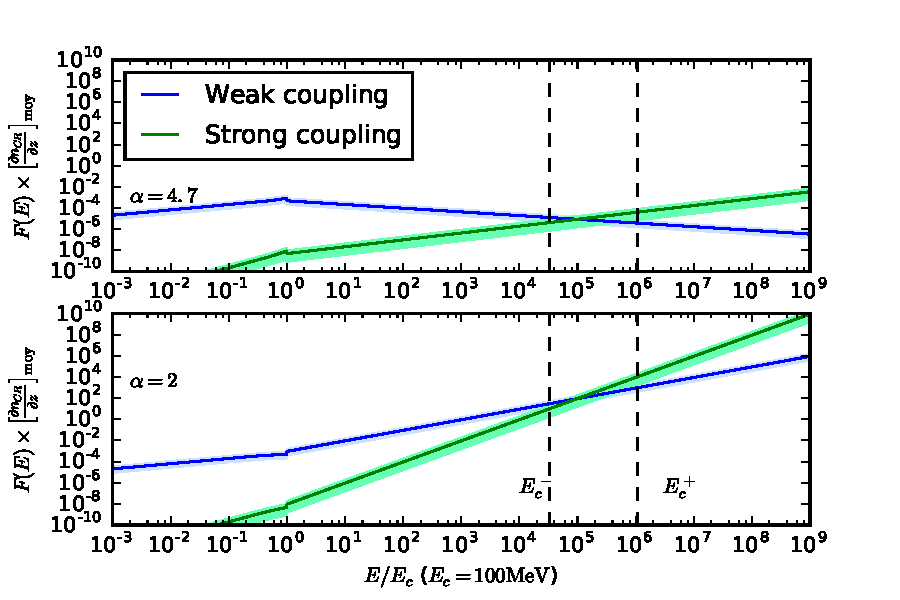
\includegraphics[width=0.3\textwidth]{./plots_progs/wnm_f(E_100MeV).pdf}
      \label{sub:WNM_100MeV}
                         }
    \subfloat[WNM - $E_c = 1~\mathrm{GeV}$]{
      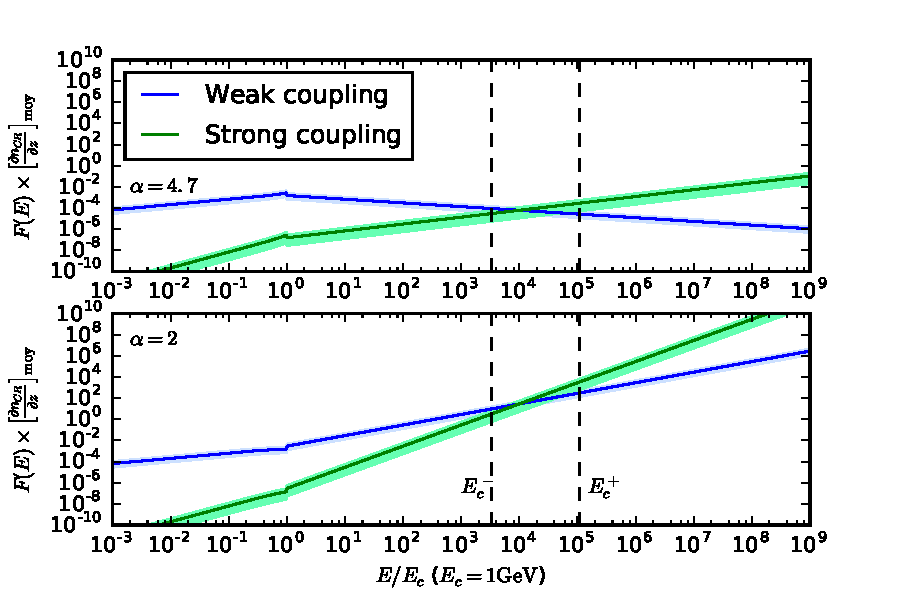
\includegraphics[width=0.3\textwidth]{./plots_progs/wnm_f(E_1GeV).pdf}
      \label{sub:WNM_1GeV}
                         }
    \subfloat[WNM - $E_c = 10~\mathrm{GeV}$]{
      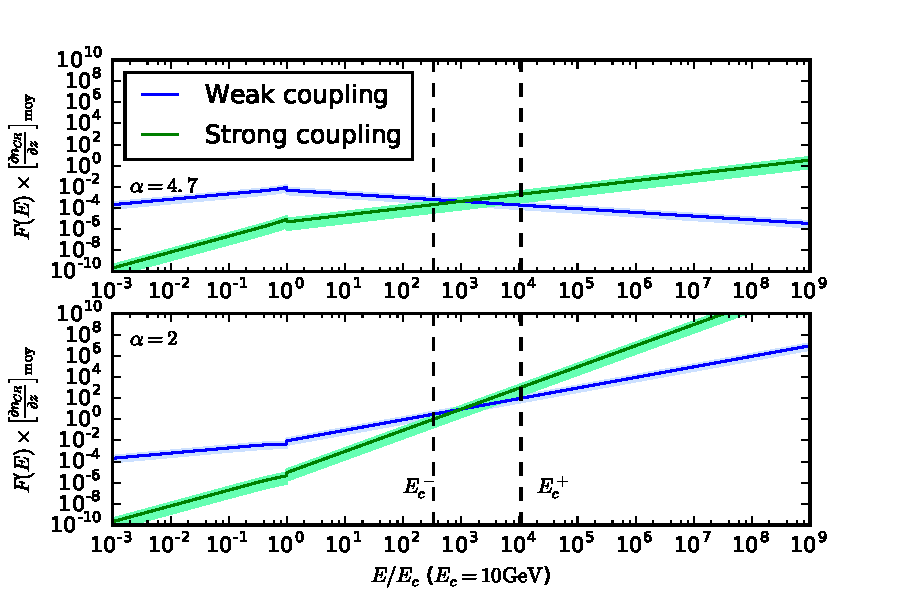
\includegraphics[width=0.3\textwidth]{./plots_progs/wnm_f(E_10GeV).pdf}
      \label{sub:WNM_10GeV}
                         } \\
    \subfloat[CNM - $E_c = 100~\mathrm{MeV}$]{
      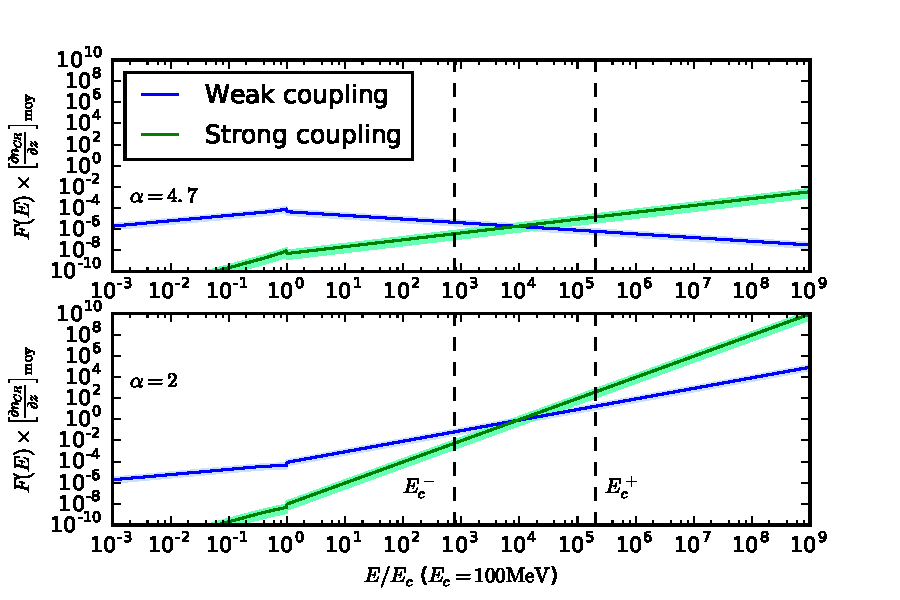
\includegraphics[width=0.3\textwidth]{./plots_progs/cnm_f(E_100MeV).pdf}
      \label{sub:popul}
                         }   
    \subfloat[CNM - $E_c = 1~\mathrm{GeV}$]{
      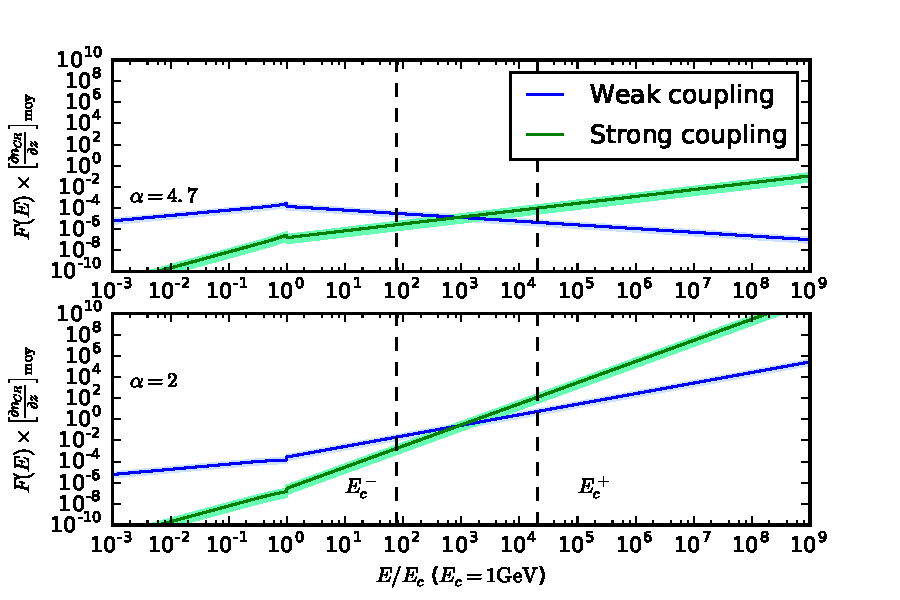
\includegraphics[width=0.3\textwidth]{./plots_progs/cnm_f(E_1GeV).pdf}
      \label{sub:popul}
                         }             
   \subfloat[CNM - $E_c = 10~\mathrm{GeV}$]{
      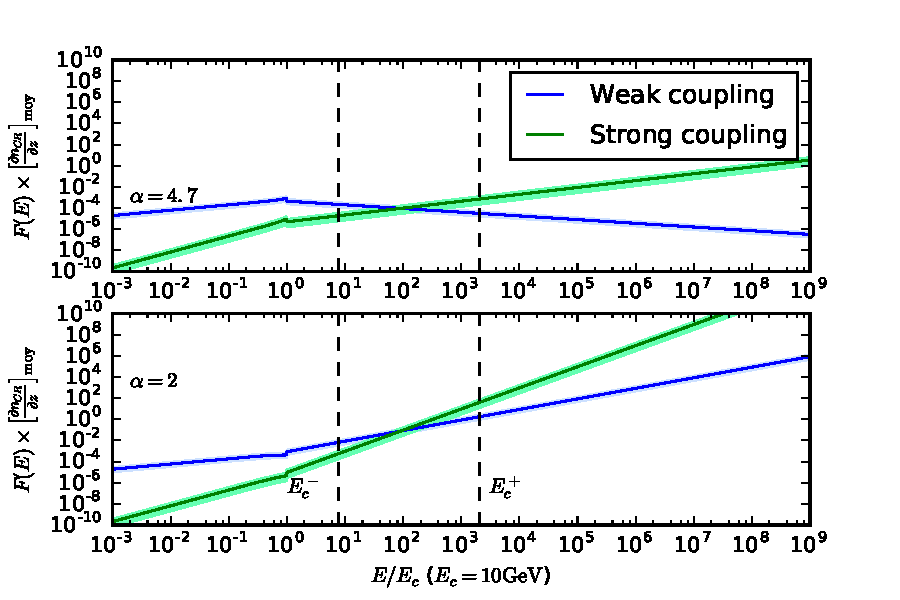
\includegraphics[width=0.3\textwidth]{./plots_progs/cnm_f(E_10GeV).pdf}
      \label{sub:popul}
                         }  \\
   \subfloat[Diffuse Cloud $E_c = 100~\mathrm{MeV}$]{
      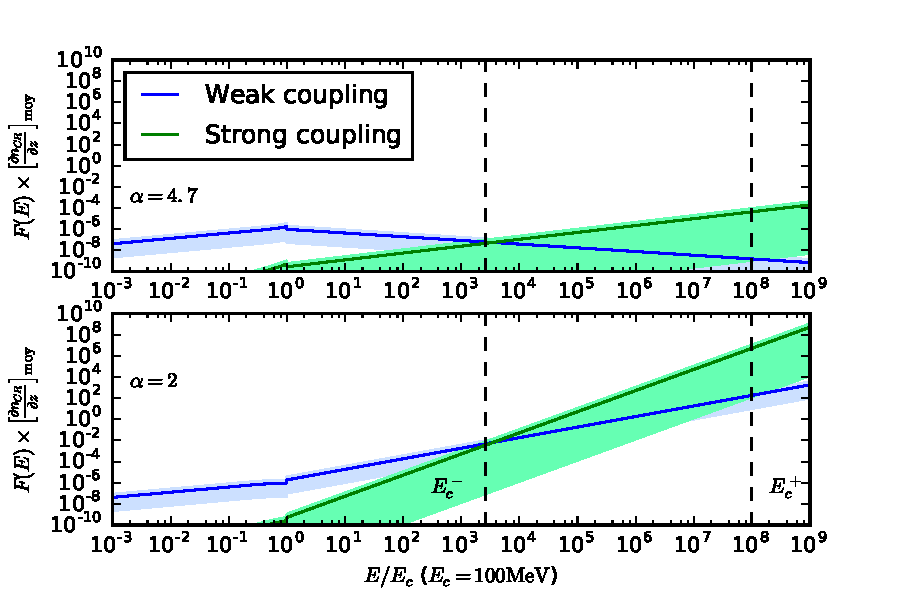
\includegraphics[width=0.3\textwidth]{./plots_progs/diffusemm_f(E_100MeV).pdf}
      \label{sub:popul}
                         }
   \subfloat[Diffuse Cloud $E_c = 1~\mathrm{GeV}$]{
      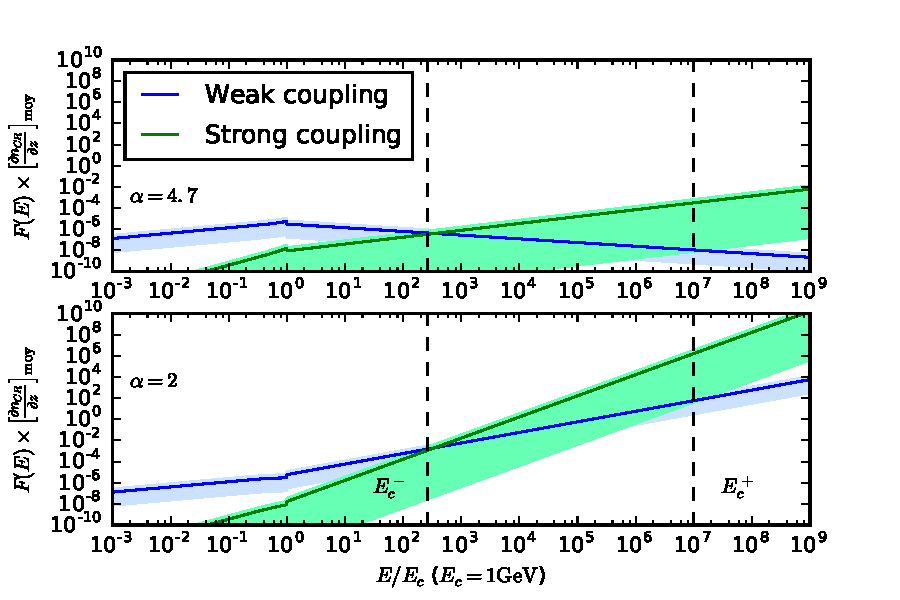
\includegraphics[width=0.3\textwidth]{./plots_progs/diffusemm_f(E_1GeV).pdf}
      \label{sub:popul}
                         }
   \subfloat[Diffuse Cloud $E_c = 10~\mathrm{GeV}$]{
      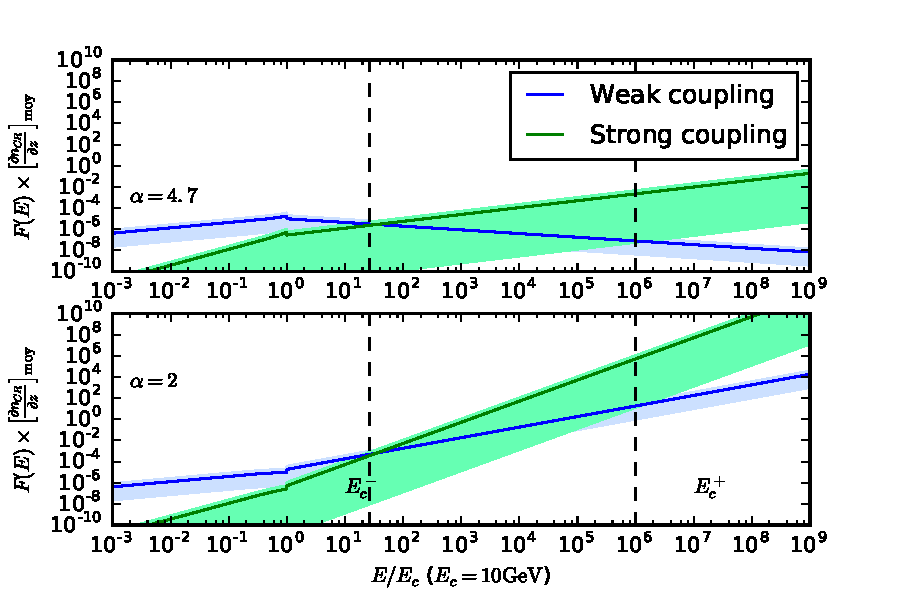
\includegraphics[width=0.3\textwidth]{./plots_progs/diffusemm_f(E_10GeV).pdf}
      \label{sub:popul}
                         } \\
   \subfloat[Dense Cloud $E_c = 100~\mathrm{MeV}$]{
      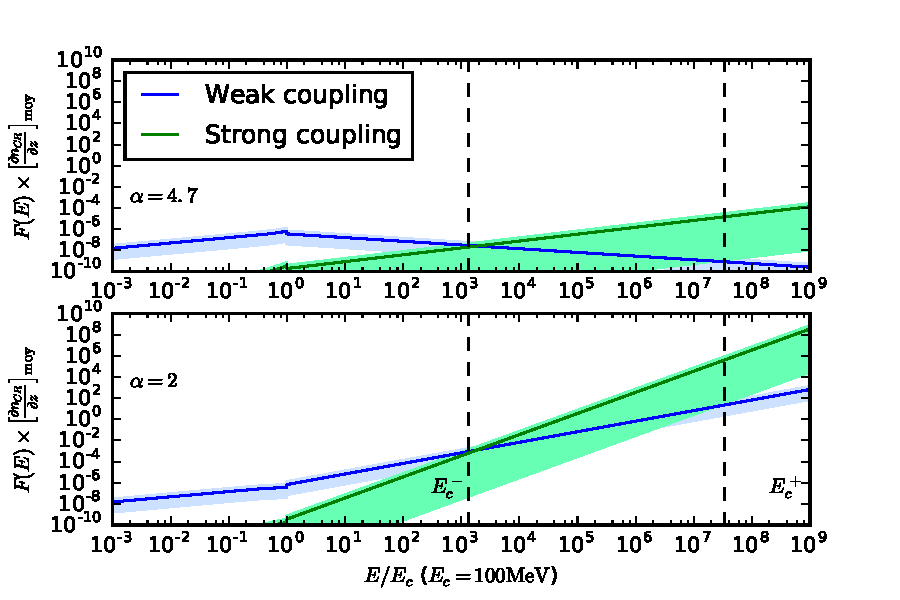
\includegraphics[width=0.3\textwidth]{./plots_progs/densemm_f(E_100MeV).pdf}
      \label{sub:popul}
                         }
   \subfloat[Dense Cloud $E_c = 1~\mathrm{GeV}$]{
      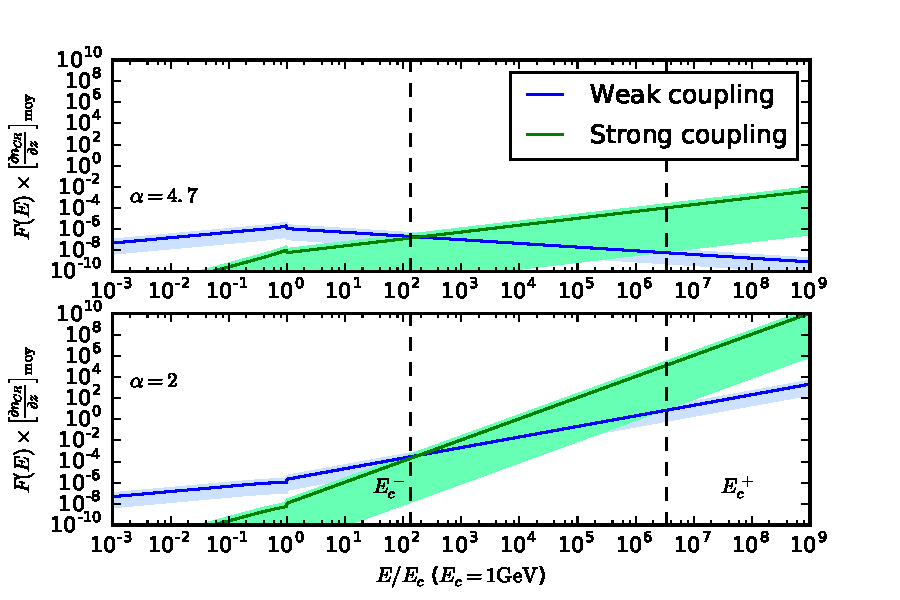
\includegraphics[width=0.3\textwidth]{./plots_progs/densemm_f(E_1GeV).pdf}
      \label{sub:popul}
                         }
   \subfloat[Dense Cloud $E_c = 10~\mathrm{GeV}$]{
      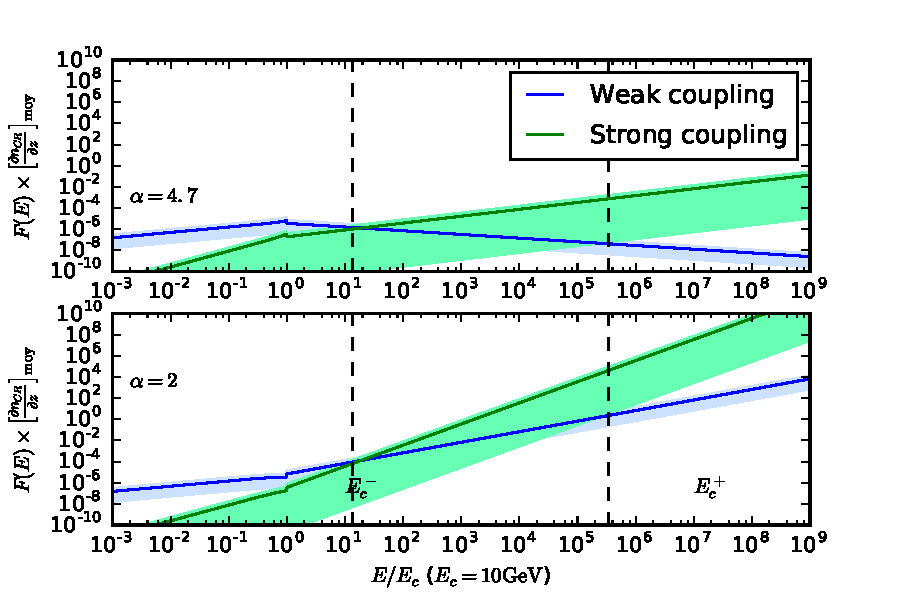
\includegraphics[width=0.3\textwidth]{./plots_progs/densemm_f(E_10GeV).pdf}
      \label{sub:popul}
                         } \\ 
   \subfloat[Dense Core $E_c = 100~\mathrm{MeV}$]{
      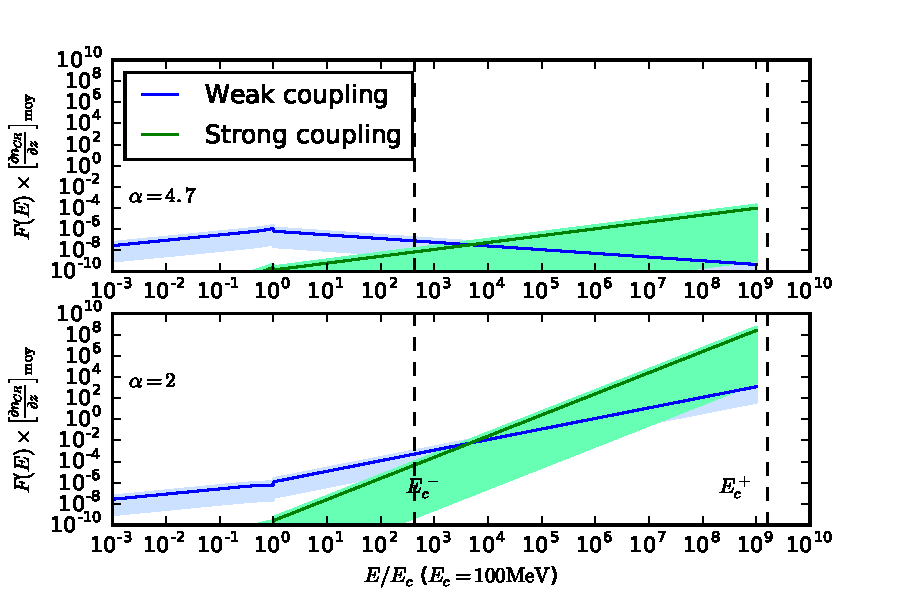
\includegraphics[width=0.3\textwidth]{./plots_progs/densecores_f(E_100MeV).pdf}
      \label{sub:popul}
                         }
   \subfloat[Dense Core $E_c = 1~\mathrm{GeV}$]{
      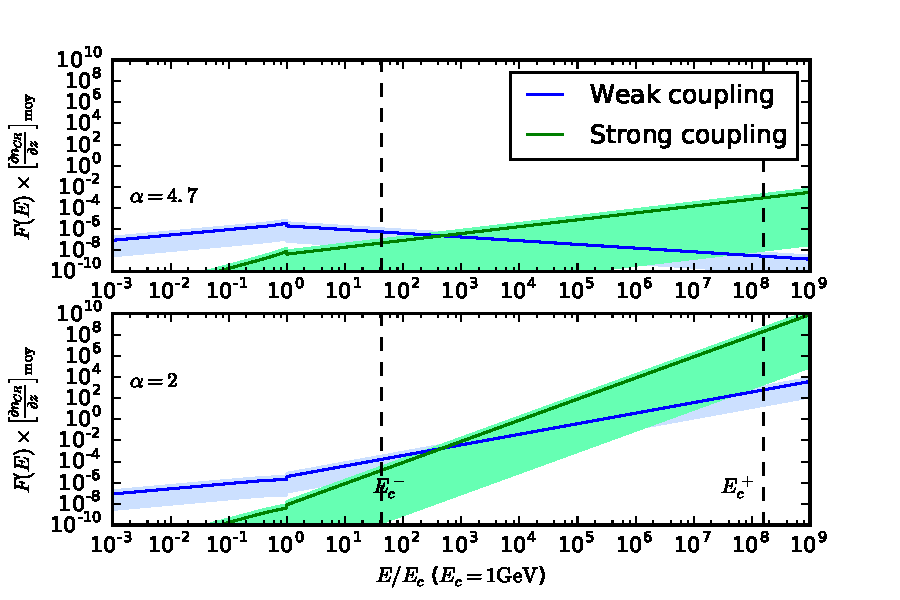
\includegraphics[width=0.3\textwidth]{./plots_progs/densecores_f(E_1GeV).pdf}
      \label{sub:popul}
                         }
   \subfloat[Dense Core $E_c = 10~\mathrm{GeV}$]{
      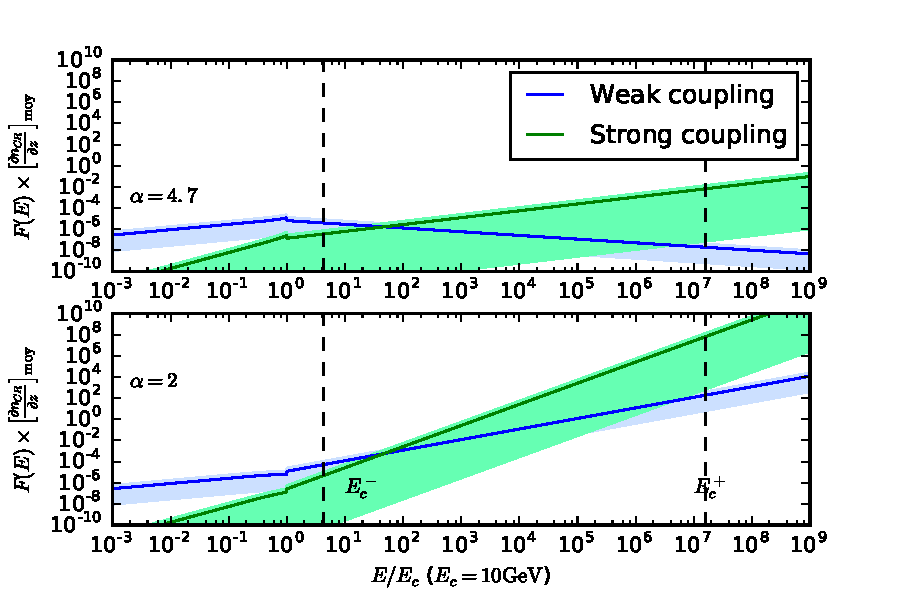
\includegraphics[width=0.3\textwidth]{./plots_progs/densecores_f(E_10GeV).pdf}
      \label{sub:popul}
                         } \\
    \caption{Exemple de fleurs de la famille des renonculacées}
    \label{fig:renonculacees}
  \end{center}
\end{figure}



\end{document}